\appendix
\section{Anexos}

Los anexos presentados a continuación contienen material gráfico complementario que respalda el desarrollo del proyecto realizado por el \textbf{Grupo 06}. Estas evidencias visuales permiten verificar la correcta implementación de la infraestructura de red, la configuración de los dispositivos, así como la ejecución de las pruebas y ataques documentados en las secciones anteriores.

Cada anexo se encuentra debidamente identificado y descrito para facilitar su análisis y correlación con los procedimientos explicados en el informe principal.

\subsection{Anexo A: Switch}

\begin{figure}[H]
\centering
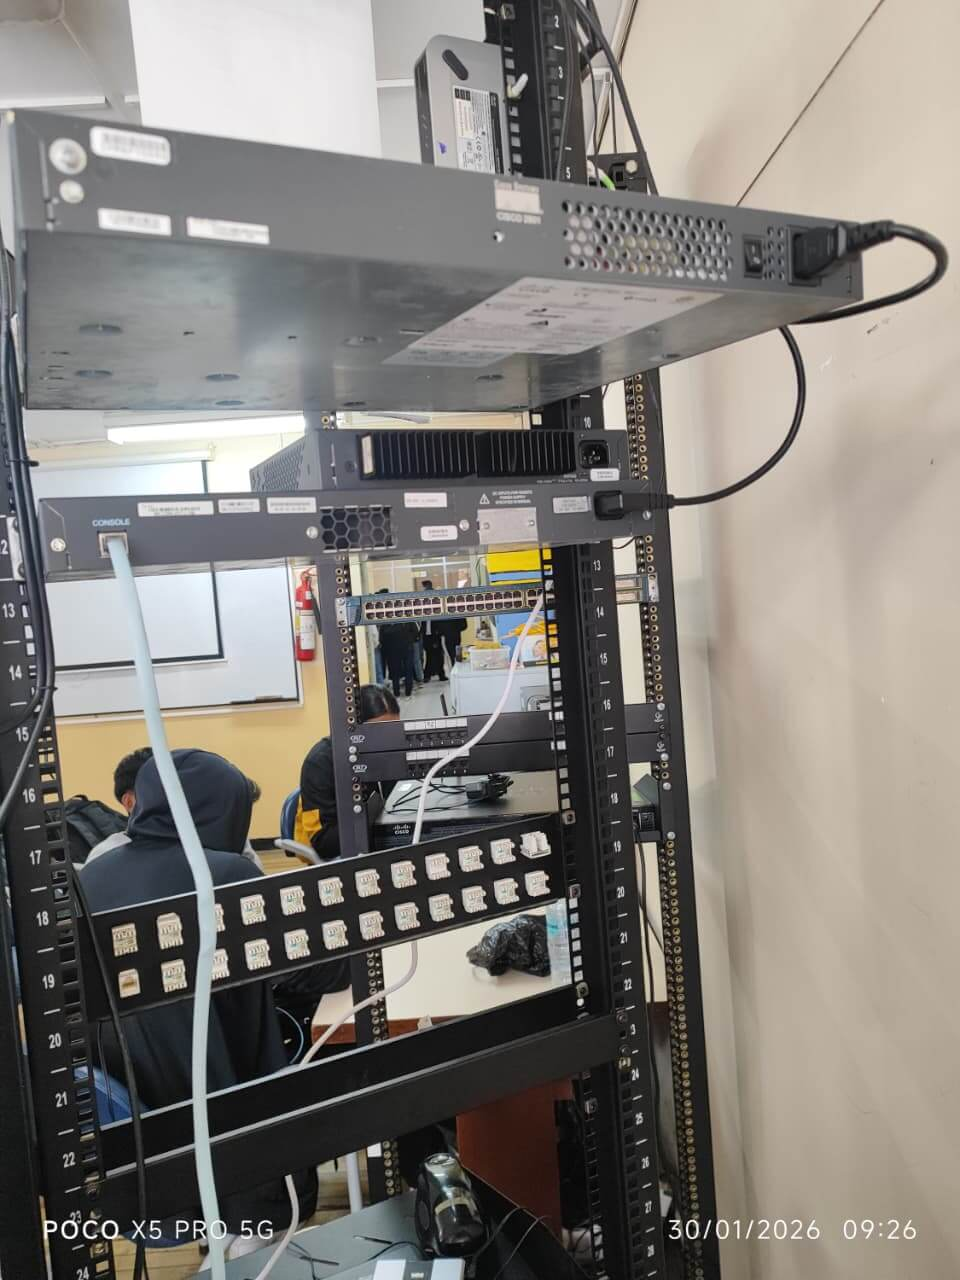
\includegraphics[width=0.85\textwidth]{assets/images/anexos/switch.jpeg}
\caption{Dispositivo Switch utilizado en la topología de red del Grupo 06}
\label{fig:switch}
\end{figure}

\subsection{Anexo B: Router}

\begin{figure}[H]
\centering
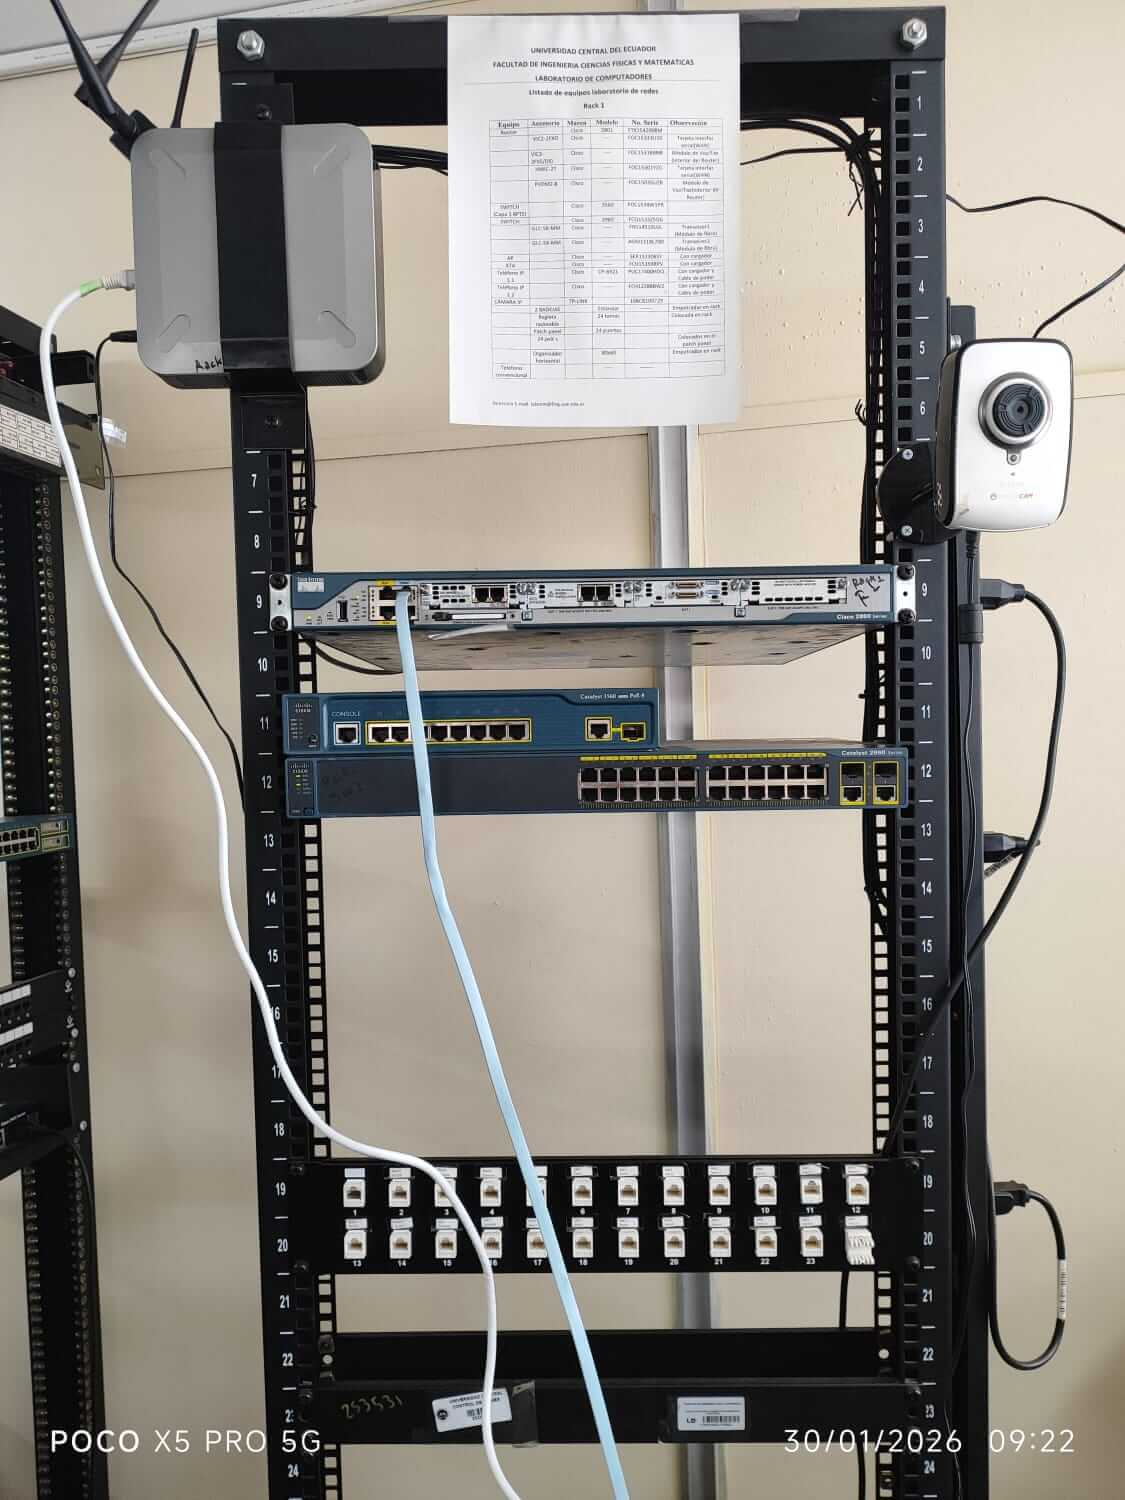
\includegraphics[width=0.85\textwidth]{assets/images/anexos/router.jpeg}
\caption{Router configurado para enrutamiento inter-VLAN}
\label{fig:router}
\end{figure}

\subsection{Anexo C: Prueba de puertos}

\begin{figure}[H]
\centering
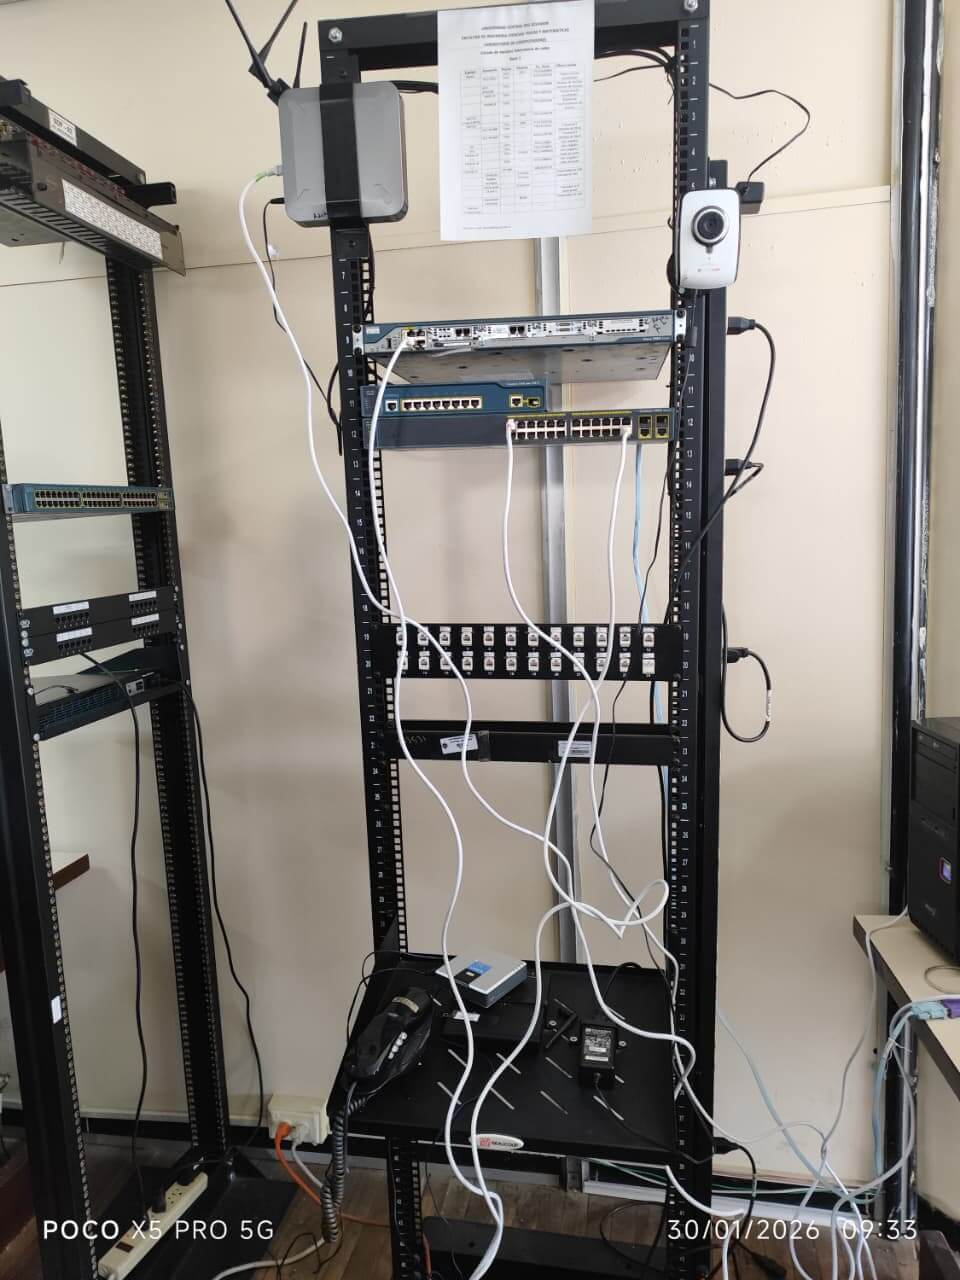
\includegraphics[width=0.9\textwidth]{assets/images/anexos/prueba_puertos.jpeg}
\caption{Resultados del escaneo y monitoreo de puertos realizado desde Kali Linux}
\label{fig:puertos}
\end{figure}

\subsection{Anexo D: Configuración de red completa}

\begin{figure}[H]
\centering
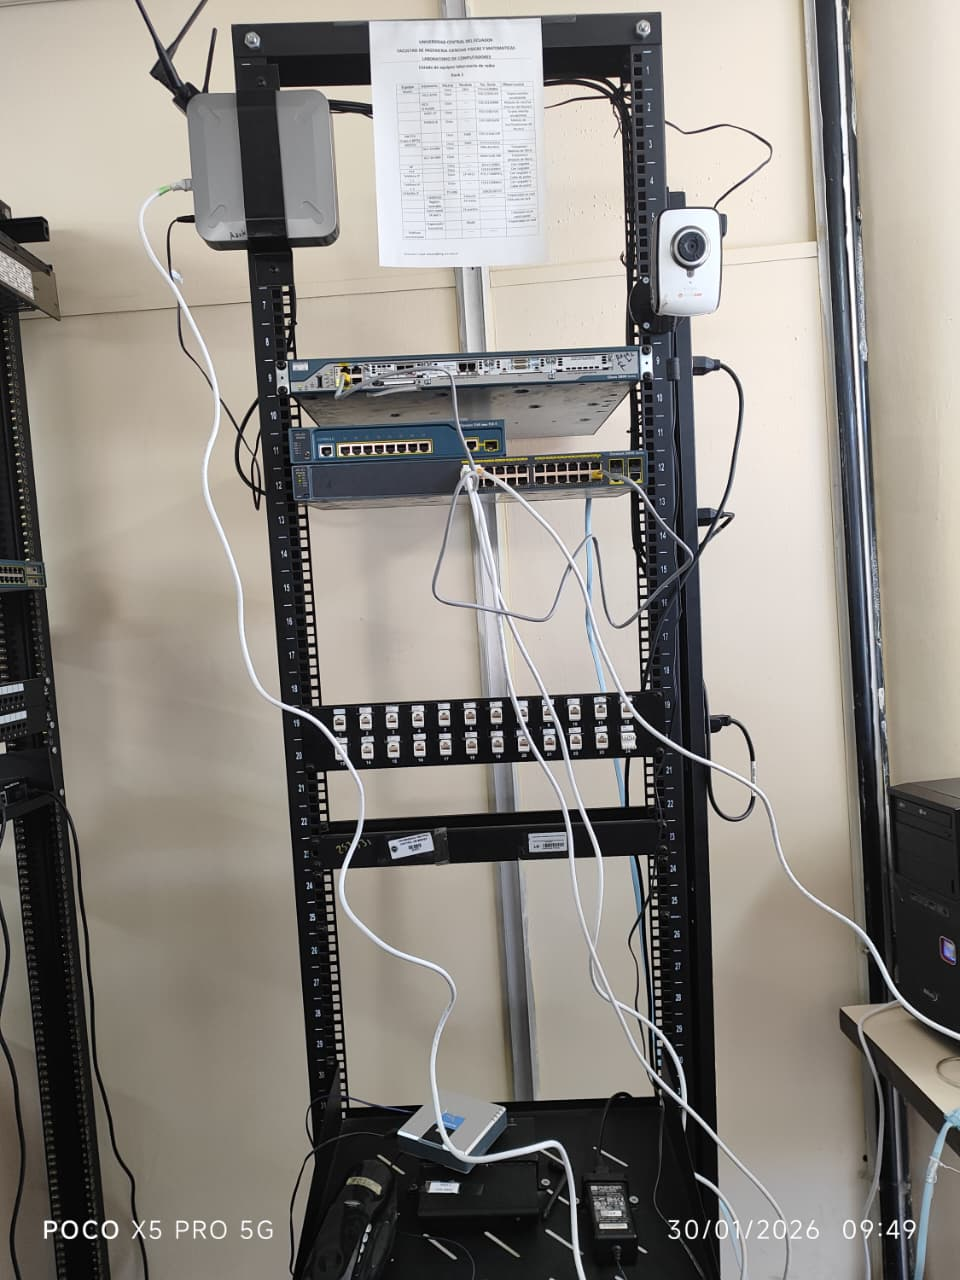
\includegraphics[width=0.95\textwidth]{assets/images/anexos/topologia_completa.jpeg}
\caption{Topología completa de la red diseñada e implementada en Packet Tracer}
\label{fig:topologia}
\end{figure}

\subsection{Anexo E: Antena Atheros}

\begin{figure}[H]
\centering
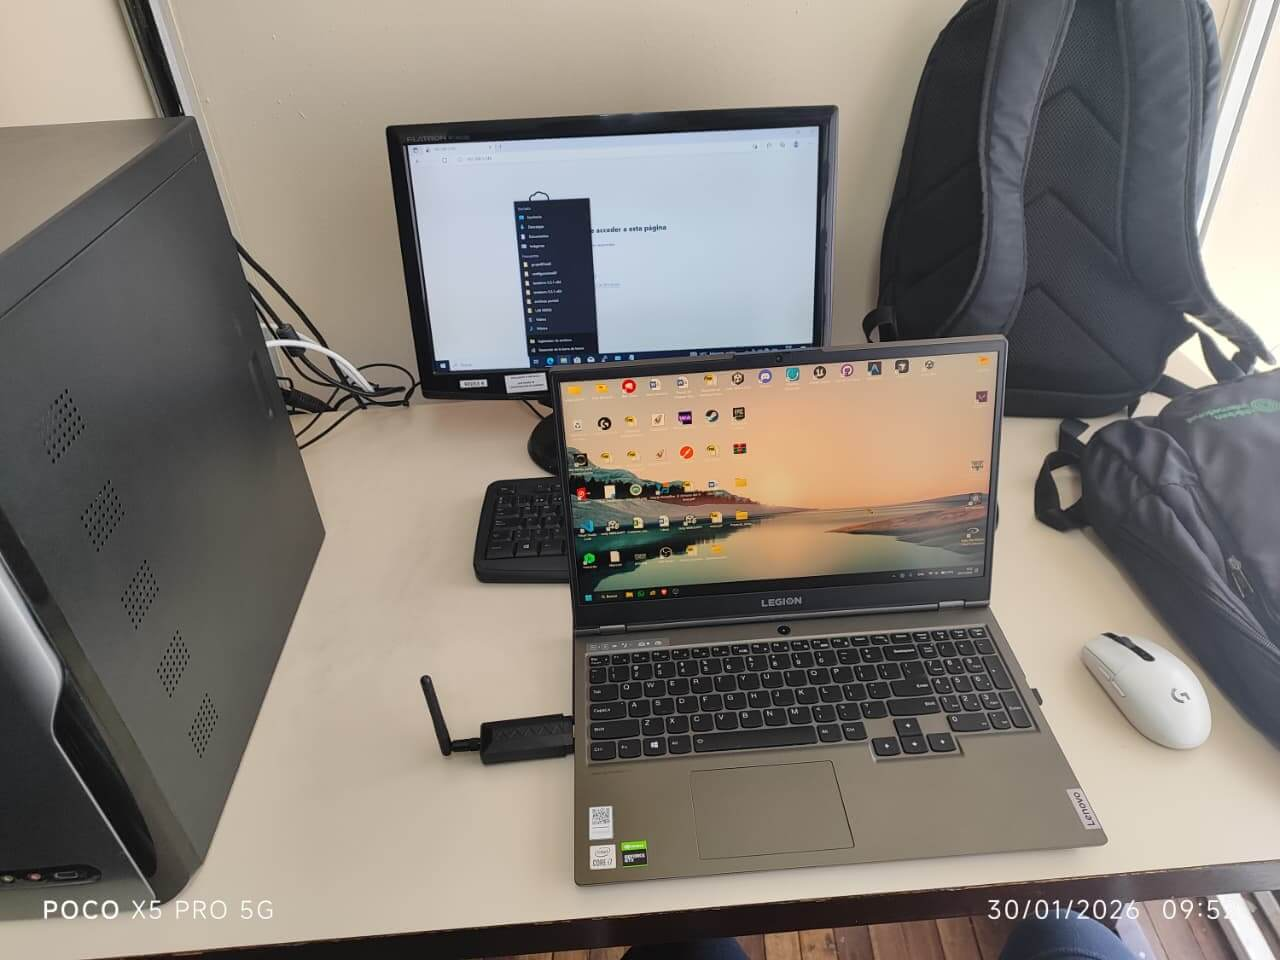
\includegraphics[width=0.75\textwidth]{assets/images/anexos/atheros.jpeg}
\caption{Antena Atheros utilizada para pruebas de auditoría WiFi}
\label{fig:atheros}
\end{figure}

\subsection{Anexo F: PC Linux (Kali Linux)}

\begin{figure}[H]
\centering
\includegraphics[width=0.85\textwidth]{assets/images/anexos/pc_kali.png}
\caption{Equipo con sistema operativo Kali Linux empleado para las pruebas de seguridad}
\label{fig:kali}
\end{figure}

\subsection{Anexo G: PC Windows Server}

\begin{figure}[H]
\centering
\includegraphics[width=0.85\textwidth]{assets/images/anexos/pc_windows_server.png}
\caption{Servidor Windows utilizado como objetivo de las pruebas de ataque}
\label{fig:windows}
\end{figure}

\subsection{Anexo H: Integrantes del Grupo 06}

\begin{figure}[H]
\centering
\includegraphics[width=0.85\textwidth]{assets/images/anexos/integrantes_grupo06.png}
\caption{Integrantes del Grupo 06 participantes en el desarrollo del proyecto}
\label{fig:grupo}
\end{figure}
